%fs
\chapter{Learning-Based Human Intention Prediction}
%\chapter{Learning}
\label{chapter:learning}
% fs


This chapter covers the learning part of this dissertation including data collecting, dataset preprocessing, and the models' structures and optimizations.

%fs
\section{Problem Description and Formulation}
%\section{Problem Introduction}

When anticipating the next action of the user, the object that the user is grasping can provide crucial information about the user's intention. Although an object detection algorithm may be helpful they can suffer from occlusion problems. Therefore, the following models attempt to solve this problem by taking an image of the user grasping a certain object and classifying which object is being grasped using the geometry of the hand.

To obtain a model that would be able to achieve the previous objective two experiments were made. In the first experiment, some types of models were tested with a smaller dataset containing only 300 images per object and 3 objects with the aim of knowing if they would be worth using and optimizing in a more complex problem. In the second experiment, a bigger dataset with 3000 images per object and 4 objects was used to train and optimize the models.

\begin{figure}[H]%[!ht]
    \centering
    \begin{tikzpicture}[>=latex']
    \tikzset{block/.style= {draw, rectangle, align=center,minimum width=3cm,minimum height=1cm},
    rblock/.style={draw, shape=rectangle,rounded corners=1.5em,align=center,minimum width=2cm,minimum height=1cm},
    input/.style={ % requires library shapes.geometric
    draw,
    trapezium,
    trapezium left angle=60,
    trapezium right angle=120,
    minimum width=2cm,
    align=center,
    minimum height=1cm
    },
    }
    
    
    \node [rblock] (camera) {Camera\\Image};
    \node [block, right =3cm of camera] (hands_keypoints) {Mediapipe\\Hands\\Model};
    \node [block, right =3cm of hands_keypoints] (body_keypoints) {Mediapipe\\Full Body\\Model};
    \node [block, below =2cm of body_keypoints] (normalization) {Points\\Normalization};
    \node [block, left =3cm of normalization] (model) {Model\\Prediction};
    \node [rblock, left =3cm of model] (output) {Predicted\\Object};

    %% paths
    \path[draw,->, text width=3cm, align=center]
                (camera) edge (hands_keypoints)
                (camera) edge[bend right] (body_keypoints)
                (hands_keypoints) edge node[above] {{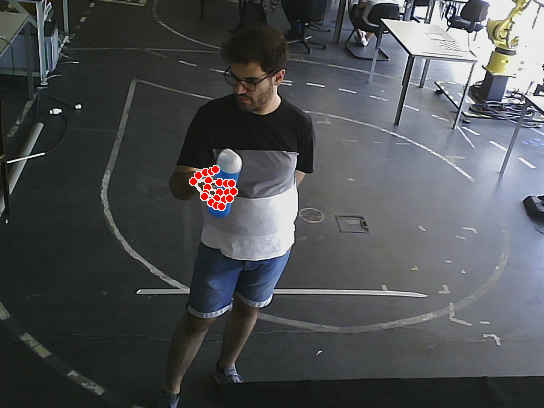
\includegraphics[width=.9\textwidth]{figs/dataset_preprocessing2_1.png}}} (body_keypoints)
                (body_keypoints) edge node[right] {right hand keypoints} (normalization) 
                (normalization) edge node[above] {normalized right hand keypoints} (model)
                (model) edge (output)
                ;

    \if{0}
    \node [rblock] (camera) {Camera\\Image};
    \node [block, right =0.5cm of camera] (hands_keypoints) {Mediapipe\\Hands\\Model};
    \node [block, right =0.5cm of hands_keypoints] (body_keypoints) {Mediapipe\\Full Body\\Model};
    \node [block, right =0.5cm of body_keypoints] (normalization) {Points\\Normalization};
    \node [block, right =0.5cm of normalization] (model) {Model\\Prediction};
    \node [rblock, right =0.5cm of model] (output) {Predicted\\Object};

    %% paths
    \path[draw,->, text width=1.7cm, align=center]
                (camera) edge (hands_keypoints)
                (camera) edge[bend right] (body_keypoints)
                (hands_keypoints) edge (body_keypoints)
                (body_keypoints) edge (normalization) 
                (normalization) edge (model)
                (model) edge (output)
                ;
    \fi
    
\end{tikzpicture}
    \caption{Machine Learning Pipeline}
    \label{fig:ml_pipeline}
\end{figure}

%fs
\section{Data Representation}
%\section{Data}

\subsection{Data Collecting}

The first step to train a supervised machine learning model is to find a dataset. However, given that this problem is very specific the datasets had to be manually collected. For this purpose, 2 datasets were collected with both consisting of a set of videos where one person would be moving and rotating a certain object. These videos were recorded at 10 frames per second to avoid consecutive frames having similar hand poses.

\begin{figure}[H]
    \centerline{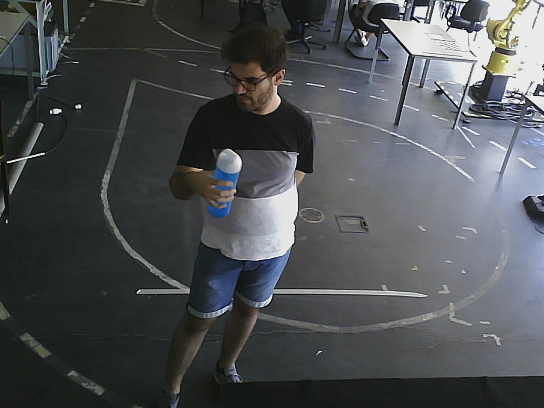
\includegraphics[width=0.49\textwidth]{figs/dataset_preprocessing1_1.png} 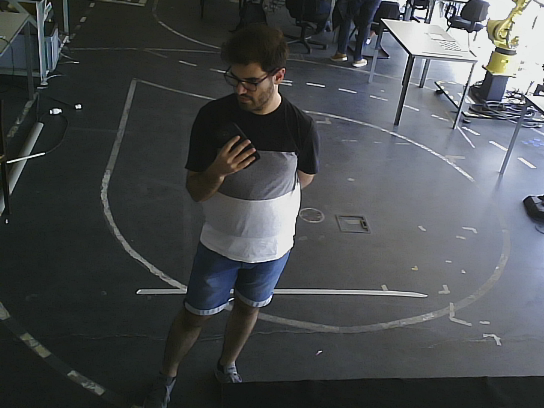
\includegraphics[width=0.49\textwidth]{figs/dataset_preprocessing1_2.png}}
    \caption[Dataset Examples]{Dataset Examples}
    \label{fig:dataset_examples}
\end{figure}

In the first dataset, 3 different objects were used (see Fig: x), and for each one, 1 person was recorded for 30 seconds resulting in 300 images per object. In the second dataset, 4 objects were used (see Fig: x), and 3 people were recorded in 4 different 25-second videos for each object resulting in 1000 frames for each person and object making it 3000 frames for each object. Recording more than one video for each combination of person and object allowed each person to grasp the object slightly differently each time in order to obtain a more diverse dataset.

\textcolor{red}{image with objects, detalhar software, metricas da aquisição mediapipe (situações com a mão visivel, manuseando o objeto, forçando a oclusão natural)}

\subsection{Dataset Preprocessing}

After having a dataset, the data had to be processed so that it would have a fitting structure to be used in the model training and testing. The images from the videos were processed using the Mediapipe hands model resulting in 21 points for each hand detected. The images were also processed by the full-body model also provided by Mediapipe so that it is possible to identify the right hand.

\begin{figure}[H]
    \centerline{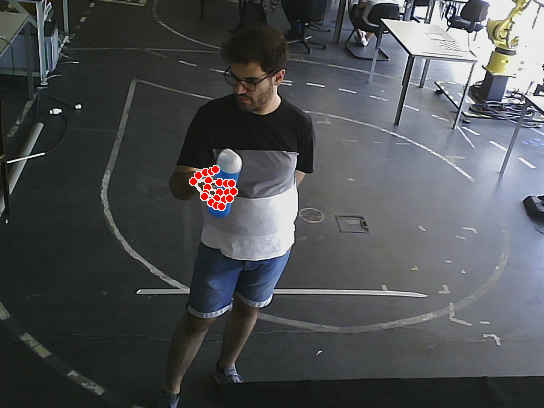
\includegraphics[width=0.49\textwidth]{figs/dataset_preprocessing2_1.png} 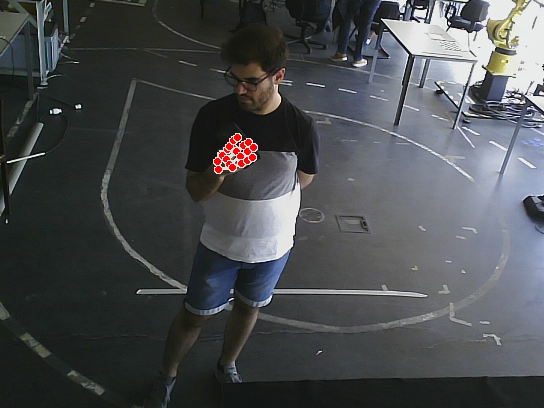
\includegraphics[width=0.49\textwidth]{figs/dataset_preprocessing2_2.png}}
    \caption[Points detected on the Pictures in Fig.~\ref{fig:dataset_examples} by Mediapipe Hands Model]{Points detected on the Pictures in Fig.~\ref{fig:dataset_examples} by Mediapipe Hands Model}
    \label{fig:dataset_examples2}
\end{figure}

These points are then subject to further processing and normalization so that the location of the hand in the image and the distance between the hand and the camera have a lesser impact. The centroid is calculated and the points are translated so that they are centered in the (0.5, 0.5, 0.5) point, the points are then scaled up as much as possible while keeping every coordinate of every point between 0 and 1.

\begin{figure}[H]
    \centerline{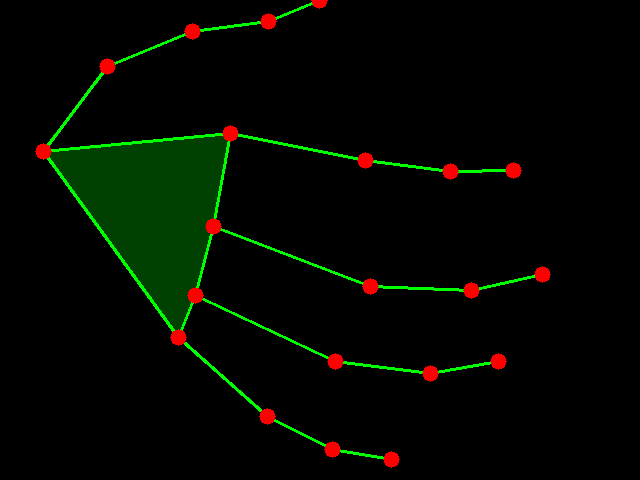
\includegraphics[width=0.49\textwidth]{figs/dataset_preprocessing3_1.png} 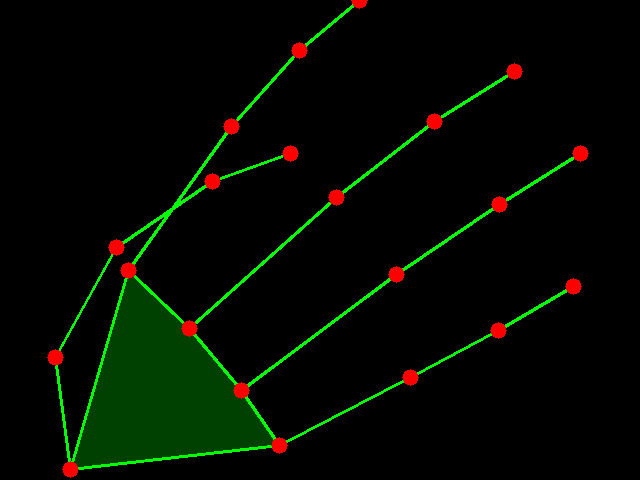
\includegraphics[width=0.49\textwidth]{figs/dataset_preprocessing3_2.png}}
    \caption[Points from the Pictures in Fig.~\ref{fig:dataset_examples2} after Normalization]{Points from the Pictures in Fig.~\ref{fig:dataset_examples2} after Normalization}
    \label{fig:dataset_examples3}
\end{figure}

\subsection{Data Splitting}

In order to train the model, the dataset was split into 3 sets: the train set (60\%), the validation set (20\%), and the test set (20\%). The random variables in the data shuffling and splitting were also fixed so that the test set is always the same, and therefore, its data is never used to train or validate the model, even in different trains. During hyperparameter optimization, the different combinations are tested using 4-fold cross-validation, which means that the model is trained 4 times, and therefore every sample of data in the initial training and validation set was used both for training and validation. Additionally, early stopping was set up so that the model would stop after 200 epochs without a better validation loss.

\section{Convolutional Neural Network}

After all the processing, each sample provided to the model is made of the 21 points that represent the right hand. Given that points are related to each other, a one-dimensional convolutional neural network was used to take advantage of this characteristic. Therefore, the CNN is responsible for taking the 21 3D points and classifying the object that is being grasped.

\subsection{Model Architecture}

When training a model with the initial architecture in the second dataset, the results were considerably lower than those achieved with the first dataset. Given that not only the dataset was bigger, but there was also one more class, it was decided that the model should have a more complex architecture, and with manual optimizations a new architecture was created which had better results. The new model can be seen on Fig.~\ref{fig:cnn_architecture} and it is made of 2 convolutional layers followed by 3 dense layers, with the third being the output layer. Between the convolutional and the dense layers and between both dense layers there is also a dropout layer so as to help with overfitting.

\begin{figure}[H]
    \centering
    {\fontsize{10}{12}\selectfont\includesvg[width=\textwidth]{figs/conv_1d_architecture.svg}}
    \caption[CNN Model Architecture]{CNN Model Architecture}
    \label{fig:cnn_architecture}
\end{figure}

\subsection{Hyperparameter Optimization}

In this model, 3 common hyperparameters in CNNs were optimized to obtain better results. These were the initial learning rate for the model training, the kernel size used by the convolutional layers and the dropout rate. Additionally, the number of convolutional layers was also tested given that, according to manual testing, it also affected the model results without changing the number of trainable parameters. The values tested for each hyperparameter can be seen on Table \ref{table:cnn_hyperparameters}.

\begin{table}[H]
    \centering
    \caption{Tested Hyperparameter Values}
    \label{table:cnn_hyperparameters}
    \begin{tabular}{|l|l|}
        \hline
        Hyperparameter & Tested Values \\
        \hline
        Learning Rate & 0.01, 0.001, 0.0001 \\
        \hline
        Number of Convolutional Layers & 1, 2, 3 \\
        \hline
        Kernel Size & 2, 3 \\
        \hline
        Dropout Rate & 0.0, 0.1, 0.2, 0.3, 0.4, 0.5 \\
        \hline
    \end{tabular}
\end{table}

In order to choose the best combination of these hyperparameters, all combinations were tested using 4-fold cross validation, which means that the model was trained 4 times, and every sample of data was used both for training and validation. It is important to note that the process to obtain these hyperparameters did not include the data from the test set. Then the average result of each combination was obtained with the combination in Table \ref{table:cnn_best_hyperparameters} having the lowest average loss with 0.2100 and an average accuracy of 94.20\%.

\begin{table}[H]
    \centering
    \caption{CNN Best Hyperparameters}
    \label{table:cnn_best_hyperparameters}
    \begin{tabular}{|l|l|}
        \hline
        Hyperparameter & Value \\
        \hline
        Learning Rate & 0.001 \\
        \hline
        Dropout & 0.5 \\
        \hline
        Kernel Size & 3 \\
        \hline
        Number of Convolutional Layers & 2 \\
        \hline
    \end{tabular}
\end{table}

\subsection{Results}

\subsubsection{First Dataset}

Initially, a simple CNN was tested and manually optimized with the first dataset resulting in the following results:

\begin{figure}[H]
    \centering
    {\fontsize{10}{12}\selectfont\includesvg[width=\textwidth]{figs/cnn_dataset1_loss_comparison.svg}}
    \caption[CNN training and validation loss evolution during training]{CNN training and validation loss evolution during training}
    \label{fig:cnn_dataset1_loss}
\end{figure}

\begin{figure}[H]
    \centering
    {\fontsize{10}{12}\selectfont\includesvg[width=\textwidth]{figs/cnn_dataset1_acc_comparison.svg}}
    \caption[CNN training and validation accuracy evolution during training]{CNN training and validation accuracy evolution during training}
    \label{fig:cnn_dataset1_acc}
\end{figure}

\begin{table}[H]
    \centering
    \caption{Metrics obtained with the First Dataset (CNN)}
    \label{table:cnn_dataset1_results}
    \begin{tabular}{|l|l|l|l|l|}
        \hline
        Metric & Test Accuracy & Precision & Recall & F1-Score \\
        \hline
        Value & 0.9551 & 0.9583 & 0.9551 & 0.9549 \\
        \hline
    \end{tabular}
\end{table}

\begin{figure}[H]
    \centering
    {\fontsize{10}{12}\selectfont\includesvg[width=0.55\textwidth]{figs/cnn_dataset1_conf_matrix.svg}}
    \caption[Confusion Matrix obtained with the First Dataset (CNN)]{Confusion Matrix obtained with the First Dataset (CNN)}
    \label{fig:cnn_dataset1_conf_matrix}
\end{figure}

Even with a relatively small dataset, this CNN shows positive results with accuracies over 95\%, so it was decided that this model should be tested in the second dataset.

\subsubsection{Second Dataset}

With the final architecture defined as well as the model hyperparameters, the final model was trained with the data of the second dataset. The Fig.~\ref{fig:cnn_loss} and Fig.~\ref{fig:cnn_acc} show the evolution of the training and validation loss and accuracy respectively during the training. According to the figures, the best validation loss occurred slightly after the 400th epoch with training stopping 200 epochs later.

\begin{figure}[H]
    \centering
    {\fontsize{10}{12}\selectfont\includesvg[width=0.98\textwidth]{figs/cnn_loss_comparison.svg}}
    \caption[CNN training and validation loss evolution during training]{CNN training and validation loss evolution during training}
    \label{fig:cnn_loss}
\end{figure}

\begin{figure}[H]
    \centering
    {\fontsize{10}{12}\selectfont\includesvg[width=0.98\textwidth]{figs/cnn_acc_comparison.svg}}
    \caption[CNN training and validation accuracy evolution during training]{CNN training and validation accuracy evolution during training}
    \label{fig:cnn_acc}
\end{figure}

With training completed, the metrics in the Table \ref{table:cnn_dataset2_results} were obtained. Given that the validation and test accuracies are close to each other we can conclude that the model managed to generalize its knowledge from the training data to classify data it has never seen before. Additionally, the confusion matrix in the Fig.~\ref{fig:cnn_dataset2_confusion_matrix} shows that the screwdriver was the object that the model managed to predict more accurately. This can be due to the fact that the hand geometry that allows a person to grasp a screwdriver intuitively is more restrict.

\begin{table}[H]
    \centering
    \caption{Metrics obtained with the Second Dataset (CNN)}
    \label{table:cnn_dataset2_results}
    \begin{tabular}{|l|l|l|l|l|}
        \hline
        Metric & Test Accuracy & Precision & Recall & F1-Score \\
        \hline
        Value & 0.9400 & 0.9403 & 0.9400 & 0.9400 \\
        \hline
    \end{tabular}
\end{table}

\begin{figure}[H]
    \centering
    {\fontsize{10}{12}\selectfont\includesvg[width=0.75\textwidth]{figs/cnn_conf_matrix.svg}}
    \caption[Confusion Matrix obtained with the Second Dataset (CNN)]{Confusion Matrix obtained with the Second Dataset (CNN)}
    \label{fig:cnn_dataset2_confusion_matrix}
\end{figure}

\section{Transformer Neural Network}

As said in Subsection \ref{subsection:transformer_neural_networks}, Transformer Neural Networks shine at capturing long-range dependencies and relationships. Therefore, considering the fact that the points obtained from Mediapipe have a specific order, we can take advantage of this ability to process structured data and effectively capture dependencies and patterns.

\subsection{Model Architecture}

The previous architecture achieved results significantly lower in the second dataset. After some manual testing, an initial layer was replaced in order to achieve better results and the number of trainable parameters was reduced when possible to allow for faster model training. The new model can be seen on Fig.~\ref{fig:transformer_architecture2} and it is made of 2 Transformer Encoder Blocks comprised of the layers shown in Fig.~\ref{fig:transformer_architecture1} followed by two sets of a Dense and a Dropout Layer and a final Dense output layer.

\begin{figure}[H]
    \centering
    {\fontsize{10}{12}\selectfont\includesvg[width=\textwidth]{figs/transformer_model_architecture.svg}}
    \caption[Tranformer Model Architecture]{Tranformer Model Architecture}
    \label{fig:transformer_architecture2}
\end{figure}

\begin{figure}[H]
    \centering
    {\fontsize{10}{12}\selectfont\includesvg[width=\textwidth]{figs/transformer_encoder.svg}}
    \caption[Transformer Encoder Block]{Transformer Encoder Block}
    \label{fig:transformer_architecture1}
\end{figure}

\subsection{Hyperparameter Optimization}

In this model, 3 hyperparameters were optimized to obtain better results. These were the initial learning rate for the model training, the dropout rate inside each transformer block, and the dropout rate of the multilayer perception at the end of the model. The values tested for each hyperparameter can be seen in Table \ref{table:transformer_hyperparameters}.

\begin{table}[H]
    \centering
    \caption{Tested Hyperparameter Values}
    \label{table:transformer_hyperparameters}
    \begin{tabular}{|l|l|}
        \hline
        Hyperparameter & Tested Values \\
        \hline
        Learning Rate & 0.01, 0.001, 0.0001 \\
        \hline
        Dropout Rate & 0.0, 0.1, 0.2, 0.3, 0.4, 0.5 \\
        \hline
        MLP Dropout Rate & 0.0, 0.1, 0.2, 0.3, 0.4, 0.5 \\
        \hline
    \end{tabular}
\end{table}

In order to choose the best combination of these hyperparameters, all combinations were
tested using 4-fold cross-validation, and the combination with the smallest average validation loss was chosen. This combination can be seen in Table \ref{table:transformer_best_hyperparameters}
having an average loss of 0.2594 and an average accuracy of 92.24\%.

\begin{table}[H]
    \centering
    \caption{Transformer Best Hyperparameters}
    \label{table:transformer_best_hyperparameters}
    \begin{tabular}{|l|l|}
        \hline
        Hyperparameter & Value \\
        \hline
        Learning Rate & 0.0001 \\
        \hline
        Dropout Rate & 0.5 \\
        \hline
        MLP Dropout Rate & 0.1 \\
        \hline
    \end{tabular}
\end{table}

\subsection{Results}

\subsubsection{First Dataset}

Initially, a Transformer architecture from \textcolor{red}{link} was tested and manually optimized with the first dataset resulting in the following results:

\begin{figure}[H]
    \centering
    {\fontsize{10}{12}\selectfont\includesvg[width=0.98\textwidth]{figs/transformer_dataset1_loss_comparison.svg}}
    \caption[Transformer training and validation loss evolution during training]{Transformer training and validation loss evolution during training}
    \label{fig:transformer_dataset1_loss}
\end{figure}

\begin{figure}[H]
    \centering
    {\fontsize{10}{12}\selectfont\includesvg[width=0.98\textwidth]{figs/transformer_dataset1_acc_comparison.svg}}
    \caption[Transformer training and validation accuracy evolution during training]{Transformer training and validation accuracy evolution during training}
    \label{fig:transformer_dataset1_acc}
\end{figure}

\begin{table}[H]
    \centering
    \caption{Metrics obtained with the First Dataset (Transformer)}
    \label{table:transformer_dataset1_results}
    \begin{tabular}{|l|l|l|l|l|}
        \hline
        Metric & Test Accuracy & Precision & Recall & F1-Score \\
        \hline
        Value & 0.8989 & 0.9163 & 0.8989 & 0.9001 \\
        \hline
    \end{tabular}
\end{table}

\begin{figure}[H]
    \centering
    {\fontsize{10}{12}\selectfont\includesvg[width=0.55\textwidth]{figs/transformer_dataset1_conf_matrix.svg}}
    \caption[Confusion Matrix obtained with the First Dataset (Transformer)]{Confusion Matrix obtained with the First Dataset (Transformer)}
    \label{fig:transformer_dataset1_confusion_matrix}
\end{figure}

Even with a relatively small dataset, this Transformer shows positive results with accuracies over 88\%. However, when considering the accuracies in each class, we can see that it has greater difficulty in distinguishing between two similar objects. Despite this, it was decided that this model should be tested in the second dataset.

\subsubsection{Second Dataset}

With the final architecture defined as well as the model hyperparameters, the final model was trained with the data of the second dataset. The Fig.~\ref{fig:transformer_loss} and Fig.~\ref{fig:transformer_acc} show the evolution of the training and validation loss and accuracy respectively during the training. According to the figures, the best validation loss occurred slightly after the 2500th epoch, with training stopping 200 epochs later.

\begin{figure}[H]
    \centering
    {\fontsize{10}{12}\selectfont\includesvg[width=0.98\textwidth]{figs/transformer_loss_comparison.svg}}
    \caption[Transformer training and validation loss evolution during training]{Transformer training and validation loss evolution during training}
    \label{fig:transformer_loss}
\end{figure}

\begin{figure}[H]
    \centering
    {\fontsize{10}{12}\selectfont\includesvg[width=0.98\textwidth]{figs/transformer_acc_comparison.svg}}
    \caption[Transformer training and validation accuracy evolution during training]{Transformer training and validation accuracy evolution during training}
    \label{fig:transformer_acc}
\end{figure}

With training completed, the metrics in the Table \ref{table:transformer_dataset2_results} were obtained. Given that the validation and test accuracies are close to each other we can conclude that the model managed to generalize its knowledge from the training data to classify data it has never seen before. Additionally, the confusion matrix in the Fig.~\ref{fig:transformer_dataset2_confusion_matrix} shows that the screwdriver was the object that the model managed to predict more accurately. This can be due to the fact that the hand geometry that allows a person to grasp a screwdriver intuitively is more restrict.

\begin{table}[H]
    \centering
    \caption{Metrics obtained with the Second Dataset (Transformer)}
    \label{table:transformer_dataset2_results}
    \begin{tabular}{|l|l|l|l|l|}
        \hline
        Metric & Test Accuracy & Precision & Recall & F1-Score \\
        \hline
        Value & 0.9244 & 0.9244 & 0.9244 & 0.9243 \\
        \hline
    \end{tabular}
\end{table}

\begin{figure}[H]
    \centering
    {\fontsize{10}{12}\selectfont\includesvg[width=0.75\textwidth]{figs/transformer_conf_matrix.svg}}
    \caption[Confusion Matrix obtained with the Second Dataset (Transformer)]{Confusion Matrix obtained with the Second\\Dataset (Transformer)}
    \label{fig:transformer_dataset2_confusion_matrix}
\end{figure}

\section{Models Comparison}

In order to further test the models' ability to generalize, two additional tests were made. Taking the optimized models described in the previous section, firstly, they were tested using only data recorded with one user, and then they were tested using one user for testing and the other two for the training phase. 

\subsubsection{First Case}

\begin{table}[H]
    \centering
    \caption{First Case Results}
    \label{table:results_first_case}
    \begin{tabular}{|l|l|l|l|l|}
        \hline
        Model & Test Accuracy & Precision & Recall & F1-Score \\
        \hline
        CNN & 0.9244 & 0.9244 & 0.9244 & 0.9243 \\
        \hline
        Transformer & 0.9244 & 0.9244 & 0.9244 & 0.9243 \\
        \hline
    \end{tabular}
\end{table}

\subsubsection{Second Case}

Table \ref{table:results_second_case_acc} shows the results of the first test.

\begin{table}[H]
    \centering
    \caption{Accuracy Results in the Second Case}
    \label{table:results_second_case_acc}
    \begin{tabular}{|l|l|l|l|l|}
        \hline
        Model & User1 & User2 & User3 & Average \\
        \hline
        CNN & 0.9673 & 0.9243 & 0.9378 & 0.9431 \\
        \hline
        Transformer & 0.9400 & 0.8892 &  0.8660 & 0.8984 \\
        \hline
    \end{tabular}
\end{table}

\begin{table}[H]
    \centering
    \caption{Precision Results in the Second Case}
    \label{table:results_second_case_precision}
    \begin{tabular}{|l|l|l|l|l|}
        \hline
        Model & User1 & User2 & User3 & Average \\
        \hline
        CNN & & & & \\
        \hline
        Transformer & 0.9404 & 0.8894 & 0.8675 & 0.8991 \\
        \hline
    \end{tabular}
\end{table}

\begin{table}[H]
    \centering
    \caption{Recall Results in the Second Case}
    \label{table:results_second_case_recall}
    \begin{tabular}{|l|l|l|l|l|}
        \hline
        Model & User1 & User2 & User3 & Average \\
        \hline
        CNN & & & & \\
        \hline
        Transformer & 0.9400 & 0.8892 & 0.8660 & 0.8984 \\
        \hline
    \end{tabular}
\end{table}

\begin{table}[H]
    \centering
    \caption{F1-Score Results in the Second Case}
    \label{table:results_second_case_f1_score}
    \begin{tabular}{|l|l|l|l|l|}
        \hline
        Model & User1 & User2 & User3 & Average \\
        \hline
        CNN & & & & \\
        \hline
        Transformer & 0.9399 & 0.8892 & 0.8663 & 0.8985 \\
        \hline
    \end{tabular}
\end{table}

These results show that when testing with only one user, the results with the CNN are similar, but those with the Transformer are slightly lower. One justification could be that even with less variety in the data, the fact that there are fewer samples of data might counterbalance that. Given that the Transformers tend to need more training data, this also justifies the difference in the accuracy.

\subsubsection{Third Case}

Table \ref{table:results_third_case_acc} shows the results of the second test.

\begin{table}[H]
    \centering
    \caption{Accuracy Results in the Third Case}
    \label{table:results_third_case_acc}
    \begin{tabular}{|l|l|l|l|l|}
        \hline
        Model & User1 & User2 & User3 & Average \\
        \hline
        CNN & 0.7958 & 0.5970 & 0.5417 & 0.6448 \\
        \hline
        Transformer & 0.7655 & 0.5686 & 0.5309 & 0.6217 \\
        \hline
    \end{tabular}
\end{table}

\begin{table}[H]
    \centering
    \caption{Precision Results in the Third Case}
    \label{table:results_third_case_precision}
    \begin{tabular}{|l|l|l|l|l|}
        \hline
        Model & User1 & User2 & User3 & Average \\
        \hline
        CNN & & & & \\
        \hline
        Transformer & 0.7808 & 0.5776 & 0.5553 & 0.6371 \\
        \hline
    \end{tabular}
\end{table}

\begin{table}[H]
    \centering
    \caption{Recall Results in the Third Case}
    \label{table:results_third_case_recall}
    \begin{tabular}{|l|l|l|l|l|}
        \hline
        Model & User1 & User2 & User3 & Average \\
        \hline
        CNN & & & & \\
        \hline
        Transformer & 0.7655 & 0.5686 & 0.5309 & 0.6217 \\
        \hline
    \end{tabular}
\end{table}

\begin{table}[H]
    \centering
    \caption{F1-Score Results in the Third Case}
    \label{table:results_third_case_f1_score}
    \begin{tabular}{|l|l|l|l|l|}
        \hline
        Model & User1 & User2 & User3 & Average \\
        \hline
        CNN & & & & \\
        \hline
        Transformer & 0.7681 & 0.5648 & 0.5312 & 0.6214 \\
        \hline
    \end{tabular}
\end{table}

These results show that testing with a user whose data was not used to train a model produces significantly lower results. This can be justified due to different people grasping objects in different ways. Additionally, given that the dataset is made of data derived from only three people, removing one from the training data significantly reduces the variety of the training data.

\section{\textcolor{red}{Integration with Previous Work}}
